%!TEX root = /Users/louis/Documents/PhD/Deliverables/Thesis/thesis.tex

\section{Epsilon Flock: A Model Migration Language}
\label{sec:flock}
Driven by the analysis presented above, a domain-specific language for model migration, Epsilon Flock (subsequently referred to as Flock), was designed and implemented. Section~\ref{subsec:flock_design} discusses the principle tenets of Flock, which include user-defined migration rules and a novel algorithm for relating source and target model elements. In Section~\ref{subsec:flock_examples}, Flock is demonstrated via application to three examples of model migration. The work described in this section has been published in \cite{rose10flock}.

\subsection{Design and Implementation}
\label{subsec:flock_design}
Flock is a rule-based transformation language that mixes declarative and imperative parts. Its style is inspired by hybrid model-to-model transformation languages such as the Atlas Transformation Language \cite{jouault05transforming} and the Epsilon Transformation Language \cite{kolovos08etl}. Flock has a compact syntax. Much of its design and implementation is focused on the runtime. The way in which Flock relates source to target elements is novel; it is neither a new- nor an existing-target relationship. Instead, elements are copied conservatively, as described in Section~\ref{subsubsec:conservative_copying}.

Like Epsilon HUTN (Section~\ref{subsec:epsilon_hutn}), Flock is built atop Epsilon, which was described in Section~\ref{subsec:epsilon}. In particular, Flock uses the Epsilon Model Connectivity layer to provide interoperability with several modelling frameworks, and the Epsilon Object Language (EOL) for specifying the imperative part of user-defined migration rules.

\subsubsection{Abstract Syntax}
\label{subsubsec:abstract_syntax}
As illustrated by Figure~\ref{fig:abstract_syntax}, Flock migration strategies are organised into modules (\texttt{Fl\-ockMo\-du\-le}). Flock modules inherit from EOL modules (\texttt{Eo\-lMod\-ule}) and hence provide language constructs for specifying user-defined operations and for re-using modules. Flock modules comprise any number of rules (\texttt{Ru\-le}). Each rule has an original metamodel type (\texttt{or\-ig\-in\-alTy\-pe}) and can optionally specify a \texttt{gu\-ard}, which is either an EOL statement or a block of EOL statements. \texttt{Mi\-gr\-ateRu\-le}s must specify an evolved metamodel type (\texttt{ev\-ol\-vedTy\-pe}) and/or a \texttt{bo\-dy} comprising a block of EOL statements.

\begin{figure}
  \centering
  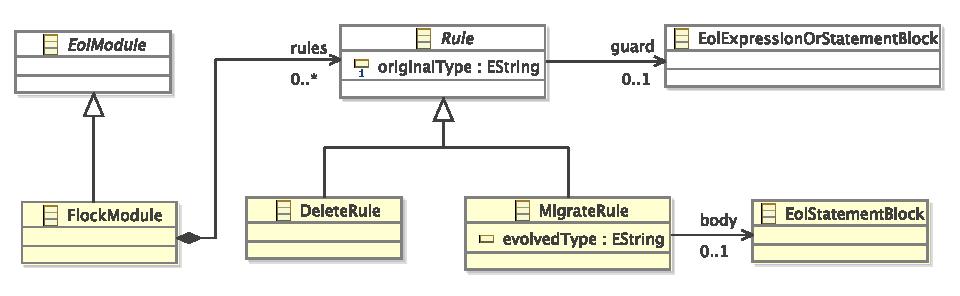
\includegraphics[scale=0.75]{5.Implementation/flock_abstract_syntax.pdf}
  \caption{The abstract syntax of Flock.}
  \label{fig:abstract_syntax}
\end{figure}

\subsubsection{Concrete Syntax}
\label{subsubsec:concrete_syntax}

Listing~\ref{lst:flock_concrete_syntax} shows the concrete syntax of migrate and delete rules. All rules begin with a keyword indicating their type (either \texttt{migrate} or \texttt{delete}), followed by the original metamodel type. Guards are specified using the \texttt{when} keywords. Migrate rules may also specify an evolved metamodel type using the \texttt{to} keyword and a \texttt{body} as a (possibly empty) sequence of EOL statements.

Note that Flock does not define a create rule. The creation of new model elements is instead encoded in the imperative part of a migrate rule specified on the containing type.

\begin{lstlisting}[float=tbp, caption=Concrete syntax of migrate and delete rules., label=lst:flock_concrete_syntax, language=Flock]
migrate <originalType> (to <evolvedType>)?
(when (:<eolExpression>)|({<eolStatement>+}))? {
	<eolStatement>*
} 

delete <originalType>
(when (:<eolExpression>)|({<eolStatement>+}))?
\end{lstlisting}

\subsubsection{Execution Semantics}
\label{subsubsec:execution_semantics}
When executed, a Flock module consumes an original model, \texttt{O}, and constructs a migrated model, \texttt{M}. The transformation is performed in three phases: rule selection, equivalence establishment and rule execution. The behaviour of each phase is described below, and the first example in Section~\ref{subsec:flock_examples} demonstrates the way in which a Flock module is executed.

\paragraph{Rule Selection}
The rule selection phase determines an \emph{applicable} rule for every model element, \texttt{e}, in \texttt{O}. As such, the result of the rule selection phase is a set of pairs of the form \texttt{<r,e>} where \texttt{r} is a migration rule.

A rule, \texttt{r}, is \emph{applicable} for a model element, \texttt{e}, when the original type of \texttt{r} is the same type as (or is a supertype of) the type of \texttt{e}; and the guard part of \texttt{r} is satisfied by \texttt{e}.

The rule selection phase has the following behaviour:

\begin{itemize}
	\item For each original model element, \texttt{e}, in \texttt{O}:
	\subitem $-$ Identify for \texttt{e} the set of all applicable rules, \texttt{R}. Order \texttt{R} by the occurrence of rules in the Flock source file.
	\subsubitem $\circ$ If \texttt{R} is empty, let \texttt{r} be a default rule, which has the type of \texttt{e} as both its original and evolved type, and an empty body.
	\subsubitem $\circ$ Otherwise, let \texttt{r} be the first element of \texttt{R}.
	\subitem $-$ Add the pair \texttt{<r,e>} to the set of selected rules.
\end{itemize}


\paragraph{Equivalence Establishment}
The equivalence establishment phase creates an equivalent model element, \texttt{e'}, in M for every pair of rules and original model elements, \texttt{<r,e>}. The equivalent establishment phase produces a set of triples of the form \texttt{<r,e,e'>}, and has the following behaviour:

\begin{itemize}
	\item For each pair \texttt{<r,e>} produced by the rule selection phase:
	\subitem $-$ If \texttt{r} is a delete rule, do nothing.
	\subitem $-$ If \texttt{r} is a migrate rule:
	\subsubitem $\circ$ Create a model element, \texttt{e'}, in M. The type of \texttt{e'} is determined from the the \texttt{evolvedType} (or the \texttt{originalType} when no \texttt{evolvedType} has been specified) of \texttt{r}.
	\subsubitem $\circ$ Copy the data contained in \texttt{e} to \texttt{e'} (using the \emph{conservative copy} algorithm described in the sequel).
	\subsubitem $\circ$ Add the triple \texttt{<r,e,e'>} to the set of equivalences.
\end{itemize}
	
\paragraph{Rule Execution}
The final phase executes the imperative part of the user-defined migration rules on the set of triples \texttt{<r,e,e'>}, and has the following behaviour:

\begin{itemize}
	\item For each triple \texttt{<r,e,e'>} produced by the equivalence establishment phase:
	\subitem $-$ Bind \texttt{e} and \texttt{e'} to EOL variables named \texttt{original} and \texttt{migrated}, respectively.
	\subitem $-$ Execute the body of \texttt{r} with EOL.
\end{itemize}


\subsubsection{Conservative Copy}
\label{subsubsec:conservative_copying}
Flock contributes an algorithm, termed \emph{conservative copy}, that copies model elements from original to migrated model only when those model elements conform to the evolved metamodel. Conservative copy is a hybrid of the new- and existing-target source-target relationships that are commonly used in M2M transformation \cite{czarnecki06survey}.

Conservative copy operates on an original model element, \texttt{e}, and its equivalent model element in the migrated model, \texttt{e'}, and has the following behaviour:

\begin{itemize}
	\item For each metafeature, \texttt{f} for which \texttt{e} has specified a value:
		\subitem $-$ Find a metafeature, \texttt{f'}, of \texttt{e'} with the same name as \texttt{f}.
			\subsubitem $\circ$ If no equivalent metafeature can be found, do nothing.
			\subsubitem $\circ$ Otherwise, copy the original value (\texttt{e.f}) to produce a migrated value (\texttt{e'.f'}) if and only if the migrated value conforms to \texttt{f'}.
\end{itemize}

The definition of conformance varies over modelling frameworks. Typically, conformance between a value, \texttt{v}, and a feature, \texttt{f}, specifies at least the following constraints:

\begin{itemize}
	\item The size of \texttt{v} must be greater than or equal to the lowerbound of \texttt{f}.
	\item The size of \texttt{v} must be less than or equal to the upperbound of \texttt{f}.
	\item The type of \texttt{v} must be the same as or a subtype of the type of \texttt{f}.
\end{itemize}


Epsilon includes a model connectivity layer (EMC), which provides a common interface for accessing and persisting models. Currently, EMC provides drivers for several modelling frameworks, permitting management of models defined with EMF, the Metadata Repository (MDR), Z or XML. To support migration between metamodels defined in heterogenous modelling frameworks, EMC was extended to include a conformance checking service, and each EMC driver to provide conformance checking semantics specific to its modelling framework. Flock implements conservative copy by delegating conformance checking responsibilities to EMC. 

Finally, some categories of model value must be converted before being copied from the original to the migrated model. Again, the need for and semantics of this conversion varies over modelling frameworks. For example, reference values typically require conversion before copying because, once copied, they must refer to elements of the migrated rather than the original model. In this case, the set of equivalences (\texttt{<r,e,e'>}) can be used to perform the conversion. In other cases, the target modelling framework must be used to perform the conversion, such as when EMF enumeration literals are copied.

 
\subsubsection{Development and User Tools}
As discussed in Section~\ref{sec:analysing_existing_techniques}, models and metamodels are typically kept separate. Flock migration strategies can be distributed by the metamodel developer in two ways. An extension point defined by Flock provides a generic user interface for migration strategy execution. Alternatively, metamodel developers can elect to build their own interface, delegating execution responsibility to \texttt{FlockModule}. The latter approach facilities interoperability with, for example, model and source code management systems.


\subsection{Examples}
\label{subsec:flock_examples}
Flock is now demonstrated using three examples of model migration. The first demonstrates the way in which a Flock module is executed and illustrates the semantics of conservative copy. The second describes the way in which the migration of the Petri net co-evolution example (introduced above) can be specified with Flock, and is included for direct comparison with the other languages discussed in Section~\ref{sec:analyis_of_languages_used_for_migration}. The final, larger example demonstrates all of the features of Flock, and is based on changes made to UML class diagrams between versions 1.5 and 2.0 of the UML specification.

\subsubsection{Process-Oriented Example}
The example presented below demonstrates, in detail, the way in which a Flock module executes a model migration strategy. Consider the original and evolved metamodels shown in Figure~\ref{fig:cc_eg_mms}, which are simplifications of two versions of the metamodel from the MDE project described in Appendix~\ref{ProcessOriented}. 

\begin{figure}
	\centering
	\subfigure[Original metamodel.]
	{
	    \label{fig:cc_eg_original}
	    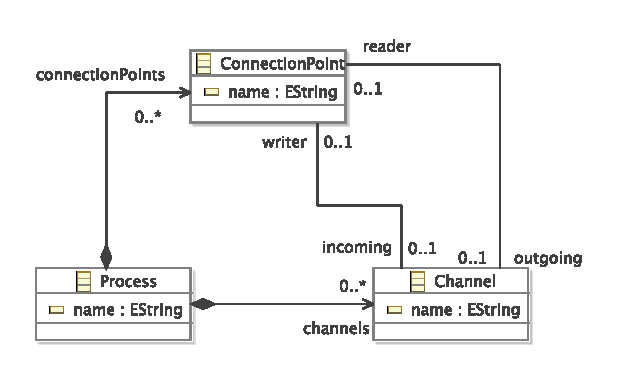
\includegraphics[width=8.5cm]{5.Implementation/images/cc_eg_original.pdf}
	}
	\subfigure[Evolved metamodel.]
	{
	    \label{fig:cc_eg_evolved}
	    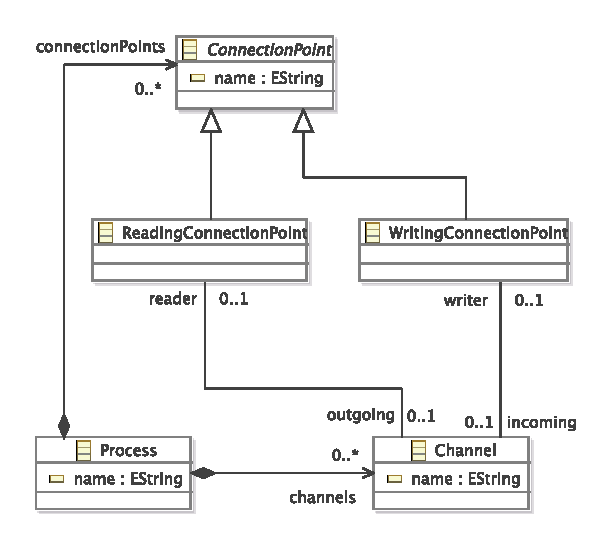
\includegraphics[width=8.5cm]{5.Implementation/images/cc_eg_evolved.pdf}
	}
	\caption{Exemplar Process-Oriented metamodel evolution}
\label{fig:cc_eg_mms}
\end{figure}

The original metamodel, shown in Figure~\ref{fig:cc_eg_original}, has been evolved to distinguish between \texttt{Co\-nn\-ec\-ti\-o\-nP\-oi\-nt}s that are a reader for a \texttt{Ch\-an\-n\-el} and \texttt{Co\-nn\-ec\-ti\-o\-nP\-oi\-nt}s that are a writer for a \texttt{Ch\-an\-n\-el} by making \texttt{Co\-nn\-ec\-ti\-o\-nP\-oi\-nt} abstract and introducing two subtypes, \texttt{Re\-a\-di\-ngCo\-nn\-ec\-ti\-o\-nP\-oi\-nt} and \texttt{Wr\-i\-ti\-ngCo\-nn\-ec\-ti\-o\-nP\-oi\-nt}, as shown in Figure~\ref{fig:cc_eg_evolved}.

Suppose that the model shown in Figure~\ref{fig:cc_eg_model}, which conforms to the original metamodel in Figure~\ref{fig:cc_eg_original} is to be migrated. The model comprises thre \texttt{Pr\-oc\-e\-ss}es named \emph{delta}, \emph{prefix} and \emph{minus}; three \texttt{Ch\-an\-n\-el}s named \emph{a}, \emph{b} and \emph{c}; and six \texttt{Co\-nn\-ec\-ti\-o\-nP\-oi\-nt}s named \emph{a?}, \emph{a!}, \emph{b?}, \emph{b!}, \emph{c?} and \emph{c!}.

\begin{figure}[htbp]
	\centering
		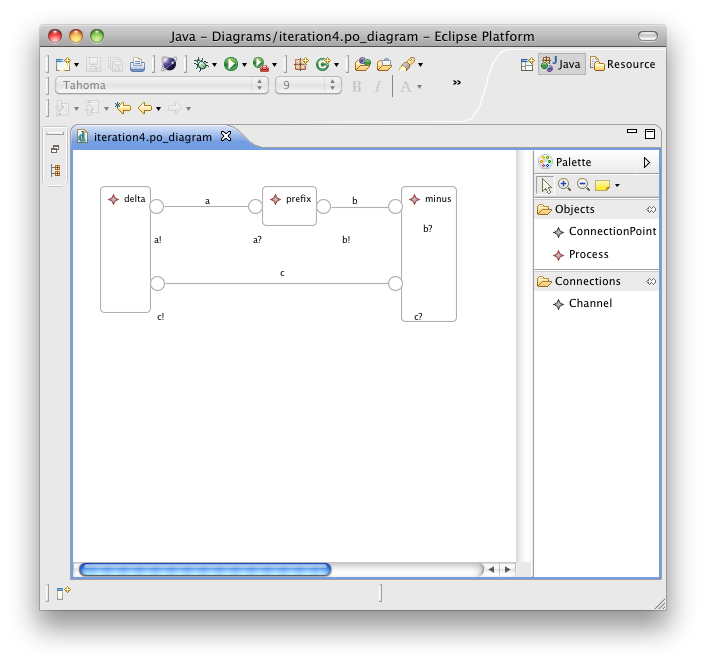
\includegraphics[scale=0.5]{A.2.ProcessOriented/images/4_model.png}
	\caption{Exemplar Process-Oriented model prior to migration}
	\label{fig:cc_eg_model}
\end{figure}

\begin{lstlisting}[float=tbp, caption=Redefining equivalences for the Component model migration., label=lst:cc_eg_rules, language=Flock]
migrate ConnectionPoint to ReadingConnectionPoint when: original.outgoing.isDefined()
migrate ConnectionPoint to WritingConnectionPoint when: original.incoming.isDefined()
\end{lstlisting}

For the migration strategy shown in Listing~\ref{lst:cc_eg_rules}, the Flock module will perform the following steps. Firstly, the rule selection phase produces a set of pairs \texttt{<r,e>}. For each \texttt{ConnectionPoint}, the guard part of the user-defined rules control which rule will be selected. \texttt{ConnectionPoint}s \texttt{a!}, \texttt{b!} and \texttt{c!} have outgoing \texttt{Channel}s (\texttt{a}, \texttt{b} and \texttt{c} respectively) and hence the migration rule on line 1 is selected. Similarly, the \texttt{ConnectionPoint}s \texttt{a?}, \texttt{b?} and \texttt{c?} have incoming \texttt{Channel}s (\texttt{a}, \texttt{b} and \texttt{c} respectively) and hence the migration rule on line 2 is selected. There is no \texttt{ConnectionPoint} with both an outgoing and an incoming \texttt{Channel}, but if there were, the first applicable rule (i.e. the rule on line 1) would be selected. For the other model elements (the \texttt{Process}es and \texttt{Channel}s) no user-defined rules are applicable, and so default rules are used instead. A default rule has an empty body and identical original and evolved types. In other words, a default rule for the \texttt{Process} type is equivalent to the user-defined rule: \texttt{migrate Process to Process \{\}}

Secondly, the equivalence establishment phase creates an element, \texttt{e'}, in the migrated model for each pair \texttt{<r,e>}. For each \texttt{ConnectionPoint}, the evolved type of the selected rule (\texttt{r}) controls the type of \texttt{e'}. The rule on line 1 of Listing~\ref{lst:cc_eg_rules} was selected for the \texttt{ConnectionPoint}s \texttt{a!}, \texttt{b!} and \texttt{c!} and hence an equivalent element of type \texttt{ReadingConnectionPoint} is created for \texttt{a!}, \texttt{b!} and \texttt{c!}. Similarly, an equivalent element of type \texttt{WritingConnectionPoint} is created for \texttt{a?}, \texttt{b?} and \texttt{c?}. For the other model elements (the \texttt{Process}es and \texttt{Channel}s) a default rule was selected, and hence the equivalent model element has the same type as the original model element.

Finally, the rule execution phase performs a conservative copy for each original and equivalent model element in the set of triples \texttt{<r,e,e'>} produced by the equivalent establishment phase. The metamodel evolution shown in Figure~\ref{fig:cc_eg_mms} has not affected the \texttt{Pr\-oc\-e\-ss} type, and hence for each \texttt{Pr\-oc\-e\-ss} in the original model, conservative copy will create a \texttt{Pr\-oc\-e\-ss} in the migrated model and copy the values of all features. For each \texttt{Ch\-an\-n\-el} in the original model, conservative copy will create an equivalent \texttt{Ch\-an\-n\-el} in the migrated model and copy the value of the \texttt{na\-me} feature from original to migrated model element. However, the values of the \texttt{re\-ad\-er} and \texttt{wr\-it\-er} features will not be copied by conservative copy because the type of these features has changed (from \texttt{Co\-nn\-ec\-ti\-o\-nP\-oi\-nt} to \texttt{Re\-a\-di\-ngCo\-nn\-ec\-ti\-o\-nP\-oi\-nt} and \texttt{Wr\-i\-ti\-ngCo\-nn\-ec\-ti\-o\-nP\-oi\-nt}, respectively). The values of the \texttt{re\-ad\-er} and \texttt{wr\-it\-er} features in the original model will not conform to the \texttt{re\-ad\-er} and \texttt{wr\-it\-er} features in the evolved metamodel. Finally, the values of the \texttt{na\-me}, \texttt{in\-co\-mi\-ng} and \texttt{ou\-tg\-oi\-ng} features of the \texttt{Co\-nn\-ec\-ti\-o\-nP\-oi\-nt} class have not evolved, and hence are copied directly from original to equivalent model elements.

The rule execution phase also executes the body of each rule, \texttt{r}, for every triple in the set \texttt{<r,e,e'>}. The user-defined rules in Listing~\ref{lst:cc_eg_rules} have no body, and hence no further execution is performed in this case.

\subsubsection{Petri Nets in Flock}
The exemplar Petri net metamodel evolution is now revisited to demonstrate the core functionality of Flock. In Listing~\ref{lst:flock}, \texttt{Net}s and \texttt{Place}s are migrated automatically. Unlike the ATL migration strategy (Listing~\ref{lst:atl}), no explicit copying rules are required. Compared to the COPE migration strategy (Listing~\ref{lst:cope}), the Flock migration strategy does not explicitly unset the original \texttt{src} and \texttt{dst} features of \texttt{Transition}.

\begin{lstlisting}[caption=Petri nets model migration in Flock, label=lst:flock, language=Flock]
migrate Transition {
  for (source in original.src) {
    var arc := new Migrated!PTArc;
    arc.src := source.equivalent();  arc.dst := migrated;
    arc.net := original.net.equivalent();
  }

  for (destination in original.dst) {
    var arc := new Migrated!TPArc;
    arc.src := migrated;  arc.dst := destination.equivalent();
    arc.net := original.net.equivalent();
  }
}
\end{lstlisting}

\subsubsection{UML Class Diagrams in Flock}
Figure~\ref{fig:uml_mms} illustrates a subset of the changes made between UML 1.5 and UML 2.0. Only class diagrams are considered, and features that did not change are omitted. In Figure~\ref{fig:original_uml_mm}, association ends and attributes are specified explicitly and separately. In Figure~\ref{fig:evolved_uml_mm}, the \texttt{Pr\-op\-er\-ty} class is used instead. The Flock migration strategy (Listing~\ref{lst:flock-uml}) for Figure~\ref{fig:uml_mms} is now discussed.

\begin{lstlisting}[caption=UML model migration in Flock, label=lst:flock-uml, language=Flock]
migrate Association {
	migrated.memberEnds := original.connections.equivalent();
}

migrate Class {
	var fs := original.features.equivalent();
	migrated.operations := fs.select(f|f.isKindOf(Operation));
	migrated.attributes := fs.select(f|f.isKindOf(Property));
	migrated.attributes.addAll(original.associations.equivalent())
}

delete StructuralFeature when: original.targetScope <> #instance

migrate Attribute to Property {
	if (original.ownerScope = #classifier) {
		migrated.isStatic = true;		
	}
}
migrate Operation {
	if (original.ownerScope = #classifier) {
		migrated.isStatic = true;
	}
}

migrate AssociationEnd to Property {
	if (original.isNavigable) {
		original.association.equivalent().navigableEnds.add(migrated)
	}
}
\end{lstlisting}

Firstly, \texttt{At\-tr\-ib\-ut\-e}s and \texttt{As\-so\-ci\-at\-i\-onEn\-d}s are now modelled as \texttt{Pr\-o\-pe\-rt\-ies} (lines 16 and 28). In addition, the \texttt{As\-so\-ci\-at\-i\-on\#na\-vi\-ga\-b\-leEn\-ds} reference replaces the \texttt{As\-so\-ci\-at\-i\-onE\-nd\#isN\-av\-ig\-ab\-le} attribute; following migration, each navigable \texttt{As\-so\-ci\-at\-i\-onE\-nd} must be referenced via the \texttt{na\-vi\-ga\-bl\-eEn\-ds} feature of its \texttt{As\-so\-ci\-at\-ion} (lines 29-31).

In UML 2.0, \texttt{St\-ru\-ct\-ur\-alFe\-at\-ur\-e\#o\-wn\-er\-Sc\-op\-e} has been replaced by \texttt{\#i\-sS\-ta\-ti\-c} (lines 17-19 and 23-25). The UML 2.0 specification states that \texttt{Sc\-op\-eKi\-nd\#cl\-as\-si\-fi\-er} should be mapped to true, and \texttt{\#i\-ns\-ta\-nce} to false. 

The UML 1.5 \texttt{St\-ru\-ct\-ur\-alFe\-at\-ur\-e\#t\-ar\-g\-et\-Sc\-op\-e} feature is no longer supported in UML 2.0, and no migration path is provided. Consequently, line 14 deletes any model element whose \texttt{t\-ar\-g\-et\-Sc\-op\-e} is not the default value.

\begin{figure}
	\centering
	\subfigure[Original metamodel.]
	{
	    \label{fig:original_uml_mm}
	    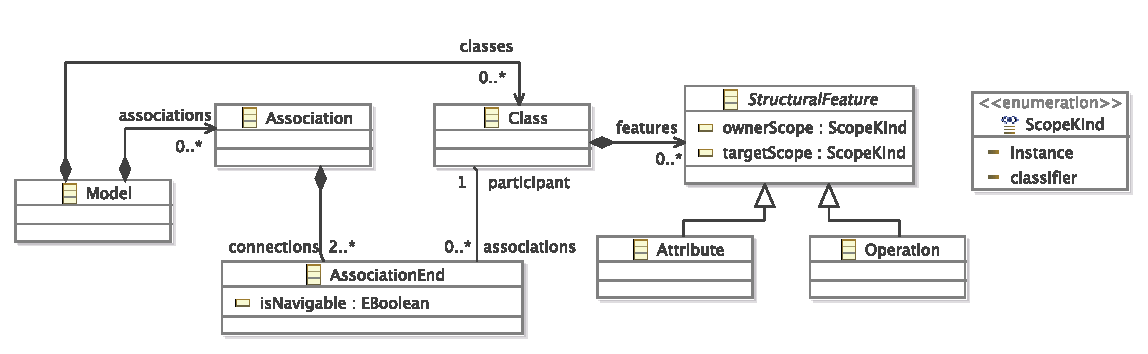
\includegraphics[width=10.5cm]{5.Implementation/images/uml_class_before.pdf}
	}
	\subfigure[Evolved metamodel.]
	{
	    \label{fig:evolved_uml_mm}
	    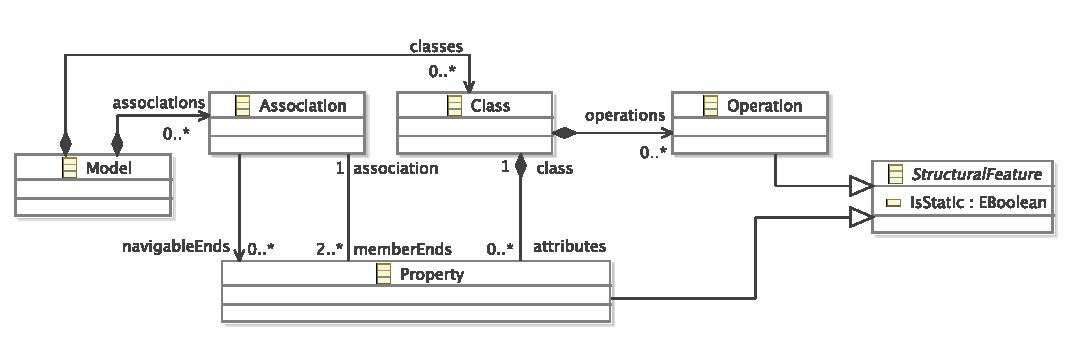
\includegraphics[width=10.5cm]{5.Implementation/images/uml_class_after.pdf}
	}
	\caption{Exemplar UML metamodel evolution}
\label{fig:uml_mms}
\end{figure}

Finally, \texttt{C\-la\-ss\#fe\-at\-ur\-es} has been split to form \texttt{C\-la\-ss\#op\-er\-at\-io\-ns} and \texttt{\#at\-tr\-ib\-ut\-es}. Lines 8 and 10 partition features on the original \texttt{Cl\-a\-ss}. \texttt{Cl\-as\-s\#a\-ss\-oc\-ia\-ti\-on\-s} has been removed in UML 2.0, and \texttt{As\-so\-ci\-at\-i\-onEn\-d}s are instead stored in \texttt{Cl\-a\-ss\#at\-tr\-ib\-ut\-es} (line 11).


\subsubsection{Summary}
Table~\ref{tab:differences} illustrates several characterising differences between Flock and the related languages presented in Section~\ref{sec:analyis_of_languages_used_for_migration}. Due to its conservative copying algorithm, Flock is the only language to provide both automatic copying and unsetting. The evaluation presented in Section~\ref{sec:quantitive} explores the extent to which automatic copying and unsetting affect the conciseness of migration strategies.

All of the approaches considered in Table~\ref{tab:differences} support EMF, arguably the most widely used modelling framework. The Ecore2Ecore approach, however, requires migration to be encoded at the level of the underlying model representation XMI. Both Flock and ATL support other modelling technologies, such as MDR and XML. However, ATL does not automatically copy model elements that have not been affected by metamodel changes. Therefore, migration between models of different technologies with ATL requires extra statements in the migration strategy to ensure that the conformance constraints of the target technology are satisfied. Because it delegates conformance checking to an EMC driver, Flock requires no such checks.

\begin{table}[b]
	\centering
	\begin{tabular}{|c|c|c|c|}
		\hline
		             & \multicolumn{2}{c|}{\textbf{Automatic}} & \textbf{Modelling} \\
		\textbf{Tool}& \textbf{Copy} & \textbf{Unset}          & \textbf{technologies} \\
		\hline
		Ecore2Ecore  & \tick             & \cross              & XMI                    \\
		\hline
		ATL          & \cross            & \tick               & EMF, MDR, KM3, XML     \\
		\hline
		COPE         & \tick             & \cross              & EMF                    \\
		\hline
		Flock        & \tick             & \tick               & EMF, MDR, XML, Z       \\
		\hline
	\end{tabular}
	\label{tab:differences}
	\caption{Properties of model migration approaches}
\end{table}

A more thorough examination of the similarities and differences between Flock and other migration strategy languages is provided by the evaluation presented in Chapter~\ref{Evaluation}.
